% Falta fixar as figuras, tabelas e algoritmos
% Falta retirar as labels em cada subfigure e colocar na figura maior
% Fazer gráficos ficarem em sequência
\chapter{Implementação e Resultados}
\label{cap:resultados}

\section{Introdução}

Nos capítulos anteriores, os algoritmos ITERATIVO e RECURSIVO foram introduzidos trazendo menores complexidades computacionais do que os métodos baseados em força bruta pura. Neste capítulo, será estudado o que tais complexidades representam em termos de recursos computacionais reais, ou seja, quanto tempo de processamento eles demandam na prática. 

Além disso, detalhes de implementação relevantes como teconologias e ambientes adotados são descritos. Finalmente, todo o plano de simulações será comentado e os resultados são analisados.

\section{Otimizações}

Antes de falar da implementação, é importante mostrar algumas ideias que ajudaram a reduzir ainda mais a complexidade dos algoritmos.

\subsection{Acoplamentos em Grafos}

Em Teoria dos Grafos, um acoplamento $M$ de um grafo $G=(V,E)$ é definido como um subconjunto de $E(G)$, tal que, para qualquer par de arestas $(i,j) \in M$, $i$ e $j$ não são adjacentes, ou seja, não compartilham vértices. Um acoplamento máximo $M^*$ é aquele com o maior número possível de arestas. 

A partir dessas definições, é possível extrair duas propriedades fundamentais:
\begin{enumerate}
\item Para qualquer $M$ em $G=(V,E)$, $g(v) \leq 1, \forall v \in V(G)$
\item Para qualquer $M^*$ em $G=(V,E)$, $|M^*|= \lfloor n/2 \rfloor$
\end{enumerate}

\subsection{Limitando a Iteração Sobre Conjuntos}

O Modelo de Interferência Primária, devido algumas características, não permite que nós da rede estejam participando de mais de um enlace de comunicação ao mesmo tempo. Logo, em uma rede modelada por um grafo $G=(V,E)$, um conjunto de arestas $C \subset E(G)$ é viável se, e somente se, as arestas de $C$ não comparilham vértices, ou seja, não são adjacentes entre si. 

Dada a definição da subseção anterior, um conjunto viável $C$ é um acoplamento $M$ de $G$. Portanto, o maior tamanho possível para um conjunto viável $C^*$ é o tamanho de um acoplamento máximo $M^*$, ou seja, $|C^*| = |M^*| = \lfloor n/2 \rfloor$. Com essa informação, é possível "podar" todos os vértices $C$ da árvore de combinações que tenham $|C|>n/2$. Nas figuras a seguir, a árvore referente a uma rede com $n=4$ e $m=4$ é "podada" em toda combinação $C$ com $|C| > 2$, ou seja, as buscas só são realziadas até a altura $h=2$.

\begin{figure}[ht] 
  \label{fig:otimizacao} 
  \begin{minipage}[b]{0.5\linewidth}
    \centering
    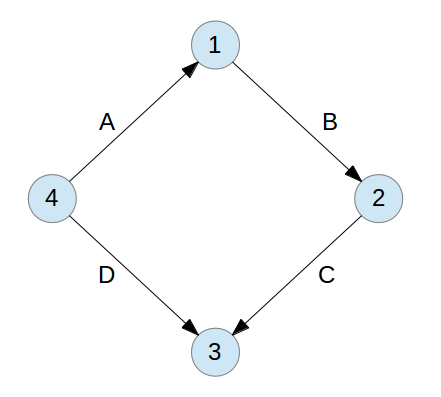
\includegraphics[width=0.5\linewidth]{figs/otim1.png} 
    \caption{Grafo com $n=m=4$} 
    \vspace{4ex}
  \end{minipage}
  \begin{minipage}[b]{0.5\linewidth}
    \centering
    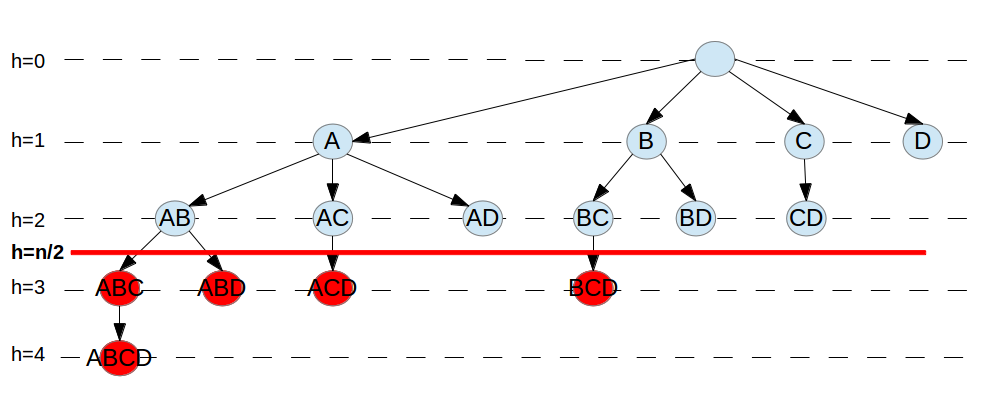
\includegraphics[width=1\linewidth]{figs/otim2.png} 
    \caption{Árvore "podada em $n/2$} 
    \vspace{4ex}
  \end{minipage} 
\end{figure}

Usando essa técnica, a complexidade para iterar sobre todos os enlaces de um conjunto C é reduzida de $O(m)$ para $O(n/2)=O(n)$.

\subsection{Reformulando o TIP}

Como consequência da definição de acoplamento, é possível reescrever o algoritmo \ref{alg:tip} com uma menor complexidade.

\begin{algorithm}[h]
	\SetVline
	{\bf input:} Conjunto de enlaces $C$\\
	\ForEach { $i \in C$}{
			\If {(($g(s_{i})>1$)$||$($g(r_{i})>1$))}{
				\Return FALSE
			}
	}
	\Return TRUE
\caption{Algoritmo TIP-G}
\label{alg:tipg}
\end{algorithm}

\subsubsection{Prova de Corretude}

Pela propriedade 1, se, dado um conjunto $C \in E(G)$, $\forall v \in V(G), g(V) \leq 1$, então C é um acoplamento e, portanto, C é viável. Isso garante que as arestas de C não compartilham vértices, ou seja, os nós do conjunto apenas participam de um enlace. Então, para testar a Interferência Primária, não é necessário verificar se em cada par de enlaces existem nós compartilhados. Basta verificar que o grau dos vértices nos enlaces de C são menores que 2. Como essa verificação é feita na linha 3, o algoritmo está correto.

\subsubsection{Análise de Complexidade}

A complexidade de espaço é a mesma do TIP original, ou seja $O(m)$. Devido a otimização apresentada na subseção anterior, sabemos que o tamanho máximo de $C$ é $n/2$ e não $m$. Portanto, reduz-se a complexidade de espaço para $O(n)$. 

No TIP original, a complexidade de tempo era $O(m^2)$ pois o algoritmo utilizava duas iterações aninhadas para testar os conjuntos. Com essa nova estrutura, é feita apenas uma iteração sobre os enlaces do conjunto C, reduzindo a complexidade para $O(m)$. Mais uma vez, como todos os enlaces de C são avaliados e $|C| \leq n/2$, então a complexidade é reduzida novamente  a $O(n)$.

\section{Detalhes de Implementação}

Todos os algoritmos aqui apresentados, bem como as estruturas de dados subjacentes, foram implementados usando a liguagem de programação C++ sob o paradigma de Orientação a Objetos. O ambiente de desenvolvimento foi composto do sistema operacional Ubuntu 16.04 64 {\it bit}s com o compilador GCC 5.4.0-6, usando o editor Atom para produção do código. O hardware utilizado foi um processador Intel Core i5-3337U com 6GB de RAM.

A primeira porção de código produzido foi referente a modelagem da rede. As classes Node, Link e Network representam os nós, enlaces e a rede, respectivamente. Além dos dados relevantes aos cálculos efetuados, como posição dos nós, potência de recepção, entre outros, vários métodos também foram criados, como geração aleaória da posição dos nós, cálculo da distância entre nós e assim por diante. O objetivo de um objeto da classe Network é servir de entrada para os algoritmos. 

Para geração das redes, três parâmetros são utilizados: (i) potência de transmissão TP; (ii) número de nós N; (iii) tamanho do lado A da área quadrada onde os nós serão dispostos. A primeira coisa a ser feita é distribuir os N nós aleatoriamente dentro da área definida por A. A distância entre todos os pares de nós é então calculada. Se a distância entre os nós for menor que um limite D, então um enlace é criado para conectá-los usando a equação \ref{eq:rp}.  

Devido algumas facilidades para gerenciar variáveis compartilhadas, os algoritmos ITERATIVO e RECURSIVO também foram codificados como classes, Iterative e Recursive, respectivamente. Ambas as classes possuem o método construtor e o método principal que implementa o algoritmo propriamente dito, além de alguns outros métodos secundários para manipulação dos dados.

A arquitetura do ambiente descrito é o principal limitante dos algoritmos. Como os processadores são de 64 {\it bit}s, o maior número inteiro nativo oferecido pela linguagem C++ é $2^{64}-1$. Portanto, até o momento, não é possível aplicar esses algoritmos a redes com mais de 64 enlaces. Devido a essa limitação, alguns cuidados também tiveram que ter sido tomados. Por exemplo, em C++, em uma contagem, ao exceder o número $2^{64}-1$, a contagem é retomada do 0. Se nenhum mecanismo para detectar essa situação fosse implantado, ao executar os algoritmos para $m=64$, o programa iria entrar em loop infinito. Um outro caso é baseado na inicialização da variável $limite$. No algoritmo ITERATIVO, $limite = 2^m$, logo, se $m=64$, então $limite=0$ e, portanto, o programa seria encerrado antes mesmo de entrar no loop principal. Mais uma vez, um mecanismo teve de ser adotado para contornar essa situação.

\section{Simulações e Resultados}

\subsubsection{Verificação da variação da quantidade de conjuntos de enlaces viáveis}

\begin{figure}[ht] 
  \label{fig:tamanho} 
  \begin{minipage}[b]{0.5\linewidth}
    \centering
    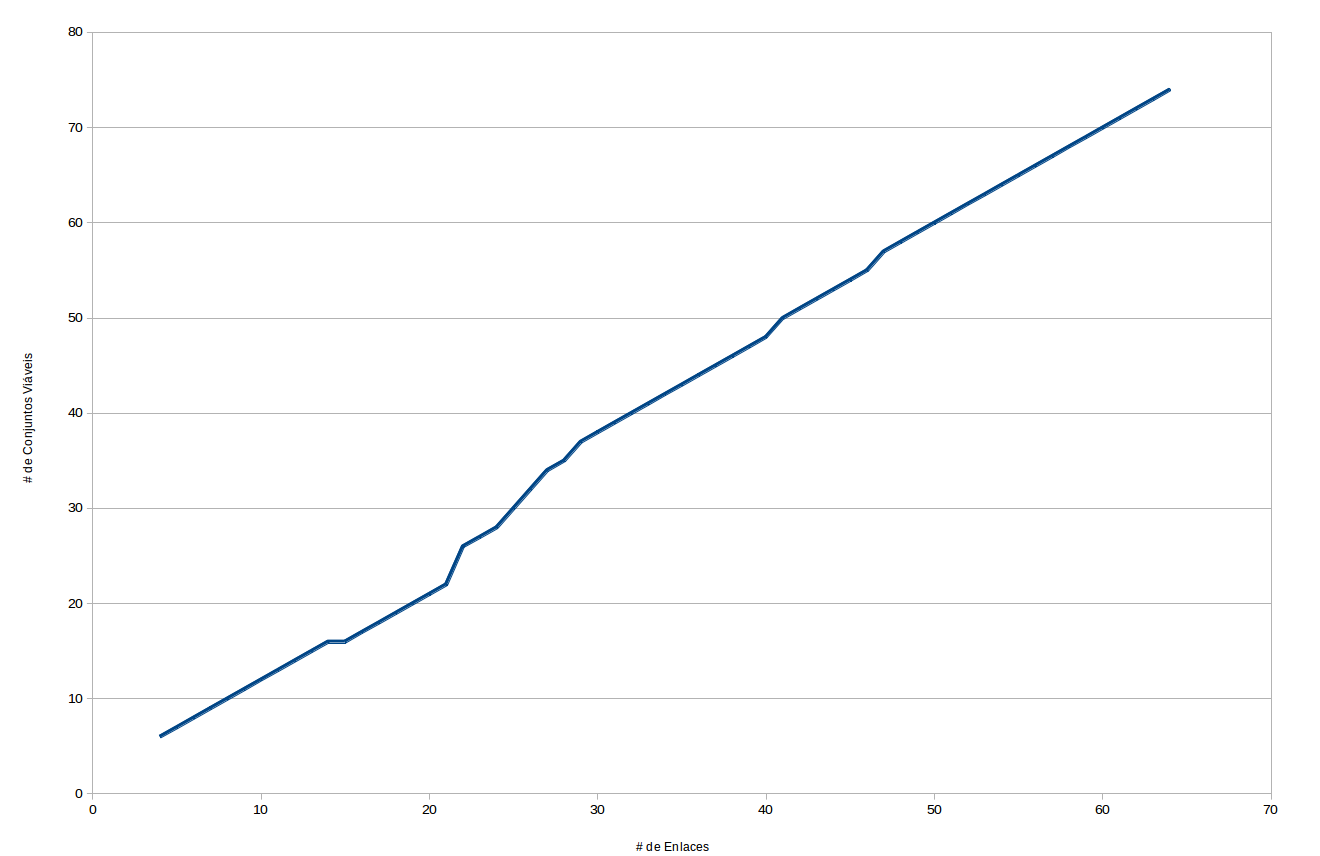
\includegraphics[width=1\linewidth]{figs/tamanho16.png} 
    \caption{Variação de $|F|$ para $n=16$} 
    \vspace{4ex}
  \end{minipage}%%
  \begin{minipage}[b]{0.5\linewidth}
    \centering
    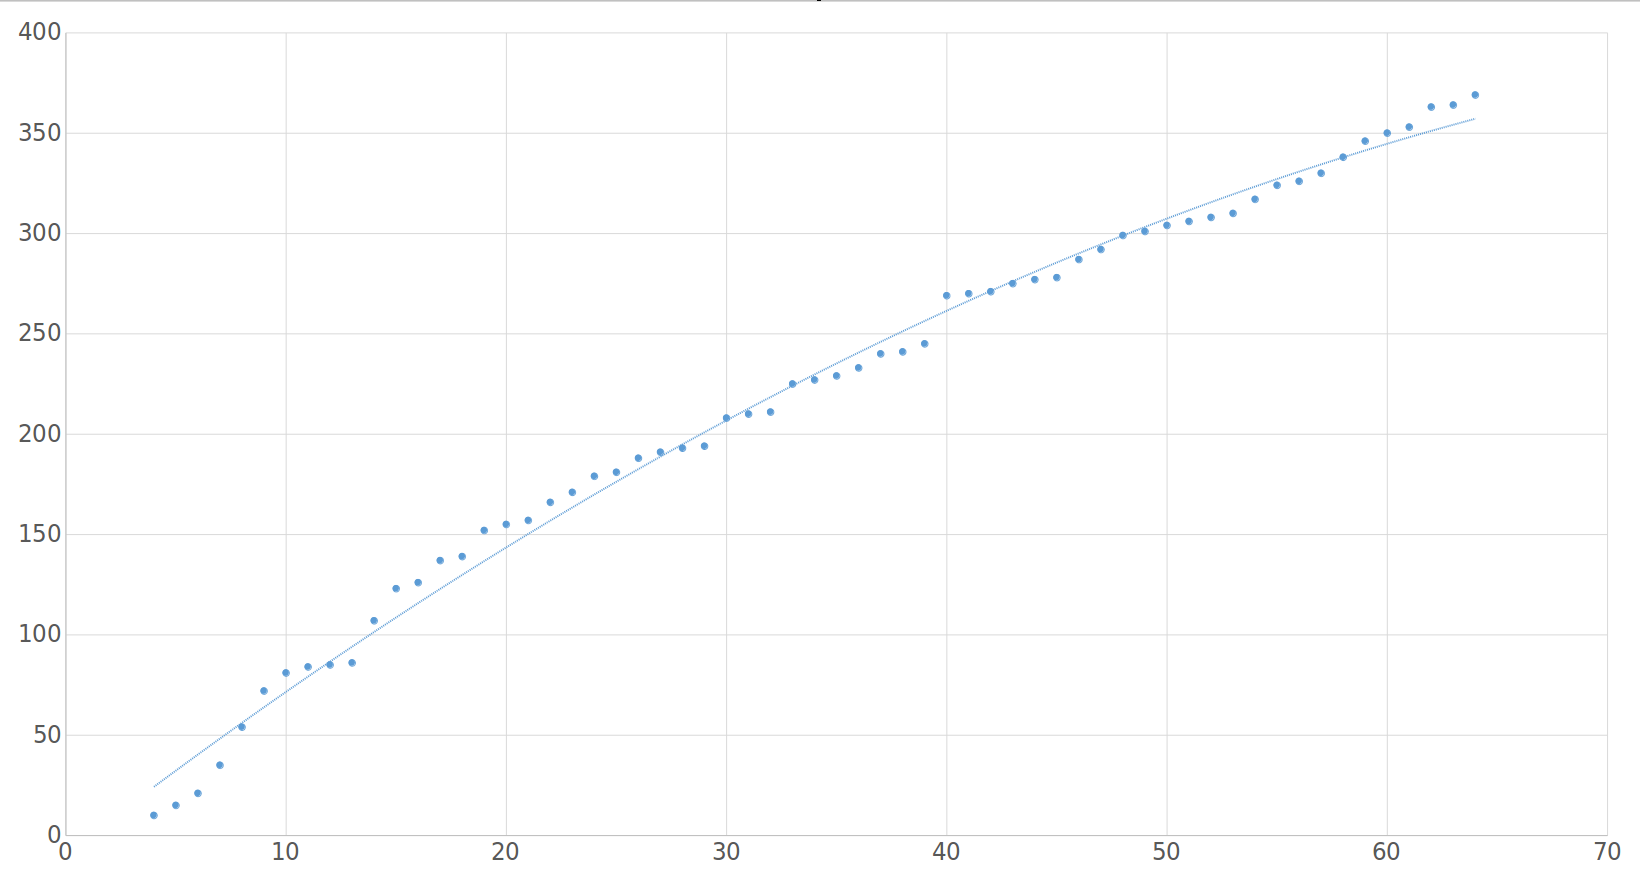
\includegraphics[width=1\linewidth]{figs/tamanho32.png} 
    \caption{Variação de $|F|$ para $n=32$} 
    \vspace{4ex}
  \end{minipage} 
  \begin{minipage}[b]{0.5\linewidth}
    \centering
    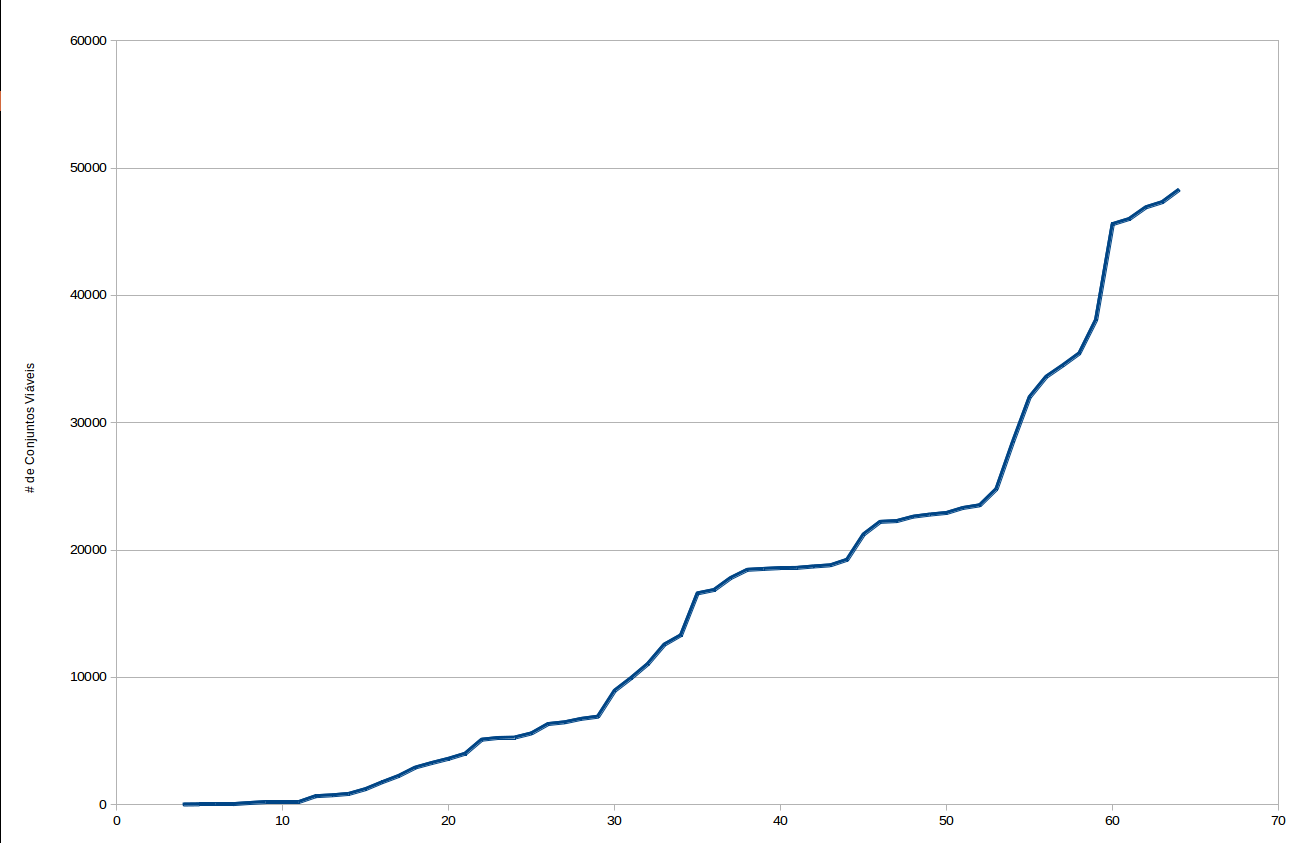
\includegraphics[width=1\linewidth]{figs/tamanho64.png} 
    \caption{Variação de $|F|$ para $n=64$} 
    \vspace{4ex}
  \end{minipage}%% 
  \begin{minipage}[b]{0.5\linewidth}
    \centering
    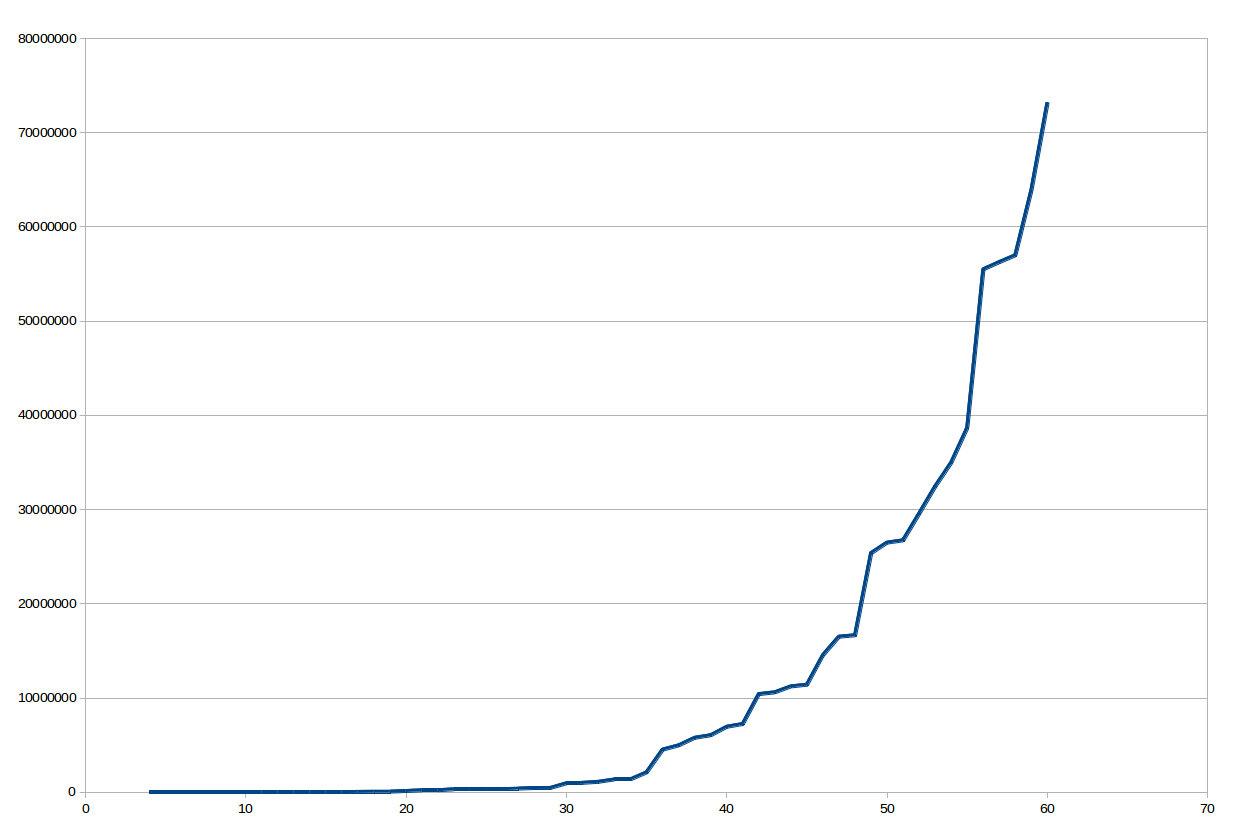
\includegraphics[width=1\linewidth]{figs/tamanho128.png} 
    \caption{Variação de $|F|$ para $n=128$} 
    \vspace{4ex}
  \end{minipage} 
\end{figure}

É importante verificar a variação da quantidade de conjuntos de enlaces viáveis resultantes da execução dos algoritmos em função do tamanho da rede para melhor determinar a sua complexidade computacional. Para isso, 30 redes diferentes para cada valor de m e n foram geradas. Foi considerado $n=\{16,32,64,128\}$. 

Em cada uma dessas redes, o número de conjuntos viáveis foi computado. A média dos valores encontrados foi utilizada para gerar uma curva e, com isso, poder aproximar a complexidade dos algoritmos.
  
Assim como no caso anterior, as curvas se acentuam com o aumento de n. Isso significa que a variação do número de conjuntos viáveis torna-se mais sensível ao aumento do número de enlaces a medida que maiores valores de n são utilizados. 

O método de regressão linear foi utilizado para interpolar as curvas subjacentes aos gráficos da figura anterior. Usando esse método, foi possível encontrar uma função  f(m) que melhor se aproxima dos pontos, ou seja, que melhor descreve o comportamento do número de conjuntos em função de m. As funções encontradas para os diferentes valores de n são mostradas na Tabela \ref{table:funcoes}.

\begin{table}[h]
\centering
\caption[Funções Aproximadas]
{Funções Aproximadas.}
\label{table:funcoes}
\begin{tabular}{lc}
\hline
$n$ & $f_n(m)$\\ \hline
16  & $f_{16}(m) = -2.11000E^-3m^2 + 1.32593m - 1.49987$\\
32  & $f_{32}(m) = -4.33900E^-2m^2 + 8.49903m - 9.00087$\\
64  & $f_{64}(m) =  1.27111E^1m^2  - 1.02108E^2m + 4.1043912E^2$\\
128 & $f_{128}(m) = 4.17002E^4m^2  - 1.77499E^6m + 1.4365315E^7$\\
\end{tabular}
\end{table}

Em todos os casos, o coeficiente de determinação $R^2$ foi superior a $93\%$. Portanto, para $n \leq 128$, a complexidade de $f_n(m)$ é $O(n^2)$. Logo, o valor de $|F|$ varia conforme a função $f_n(m)$ que, é $O(n^2)$. Consequentemente, $O(|F|)=O(n^2)$. Devido a essa aproximação, conclui-se que, as complexidades dos algoritmos ITERATIVO e RECURSIVO são, respectivamente, $O(|F|n^2) = O(n^2n^2) = O(n^4)$ e $O(|F|n) = O(n^2n) = O(n^3)$. 

\subsubsection{Resumo das Complexidades}

A Tabela \ref{table:complexidade} mostra cada algoritmo de enumeração mencionado nesse trabalho com suas respectivas complexidades computacionais.

\begin{table}[h]
\centering
\caption[Complexidades Computacionais]
{Complexidades Computacionais.}
\label{table:complexidade}
\begin{tabular}{lcc}
\hline
Algoritmo & Tempo & Espaço\\ \hline
Força Bruta Pura & $O(2^mm^2)$ & $O(2^m)$\\
BP com "Poda" (Exemplo do Capítulo \ref{cap:modelagem}) & $O(m^4)$ & $O(2^m)$\\
ITERATIVO & $O(m^4)$ & $O(m)$\\
RECURSIVO & $O(m^3)$ & $O(m)$\\
ITERATIVO + Otimizações & $O(n^4)$ & $O(m)$\\
RECURSIVO + Otimizações & $O(n^3)$ & $O(m)$\\
\end{tabular}
\end{table}

\subsubsection{Verificação do tempo de execução real dos algoritmos}

Além do tempo de execução de cada algoritmo para redes com número de enlaces compreendidos entre 4 e 64, também se mostrou importante entender o efeito da variação do número de nós. Os valores utilizados para n são $\{16, 32, 64, 128\}$. 

Então, as redes foram simuladas com diferentes valores de m e n e o tempo de execução de ambos os algoritmos foi medido. Para evitar ruídos provenientes de variações computacionais aleatórias, 30 execuções de cada algoritmo foram feitas para cada cenário, seguindo a regra de [Citar o cara que determinou esse número]. Ao final, o tempo médio das execuções foi utilizado para gerar uma curva e, com isso, poder analisar o tempo real.

\begin{figure}[ht] 
  \label{fig:tempo} 
  \begin{minipage}[b]{0.5\linewidth}
    \centering
    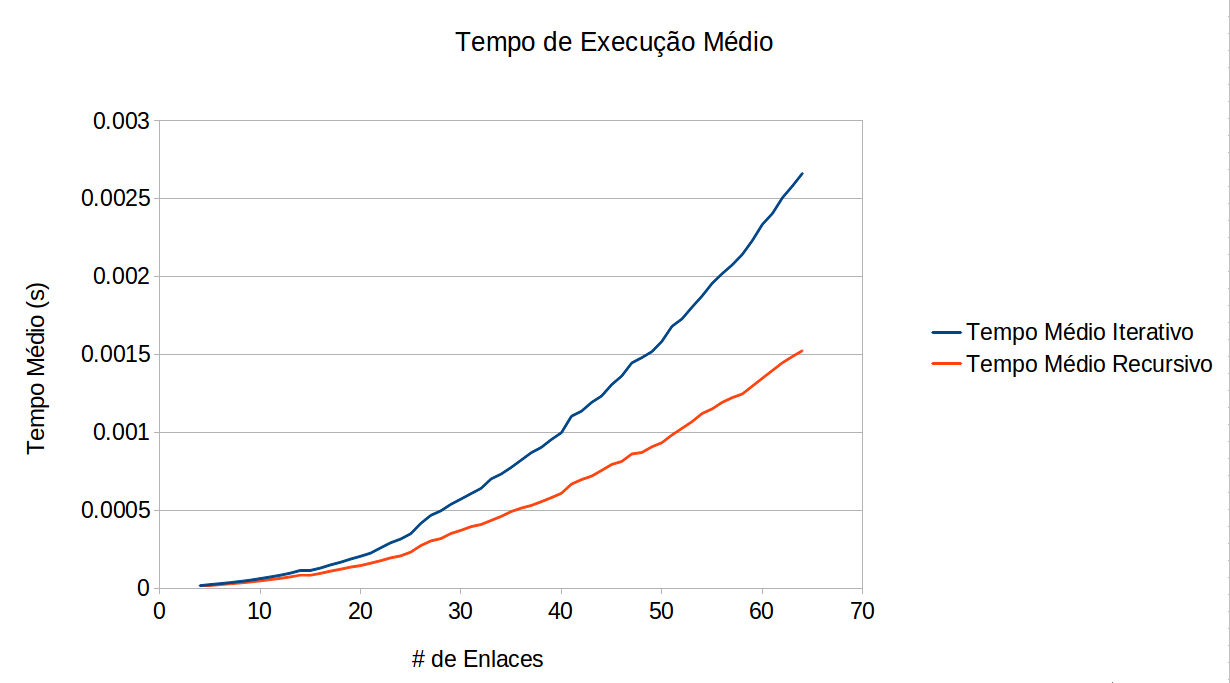
\includegraphics[width=1\linewidth]{figs/tempo16.png} 
    \caption{$n=16$} 
    \vspace{4ex}
  \end{minipage}%%
  \begin{minipage}[b]{0.5\linewidth}
    \centering
    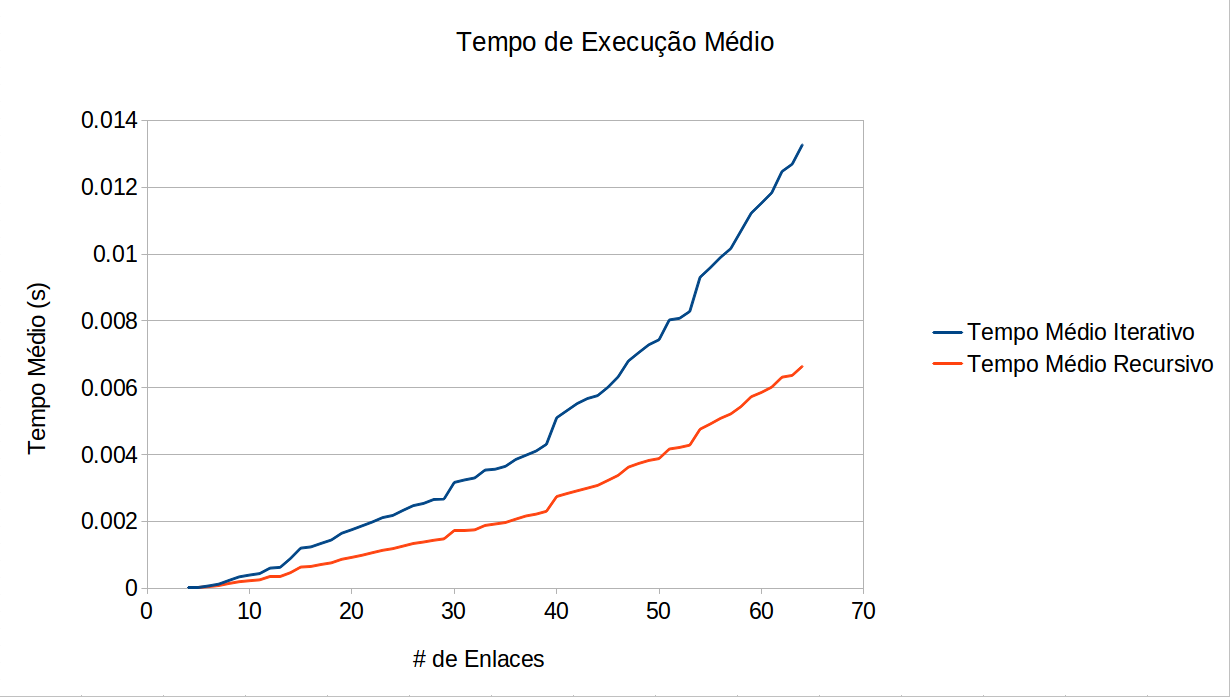
\includegraphics[width=1\linewidth]{figs/tempo32.png} 
    \caption{$n=32$} 
    \vspace{4ex}
  \end{minipage} 
  \begin{minipage}[b]{0.5\linewidth}
    \centering
    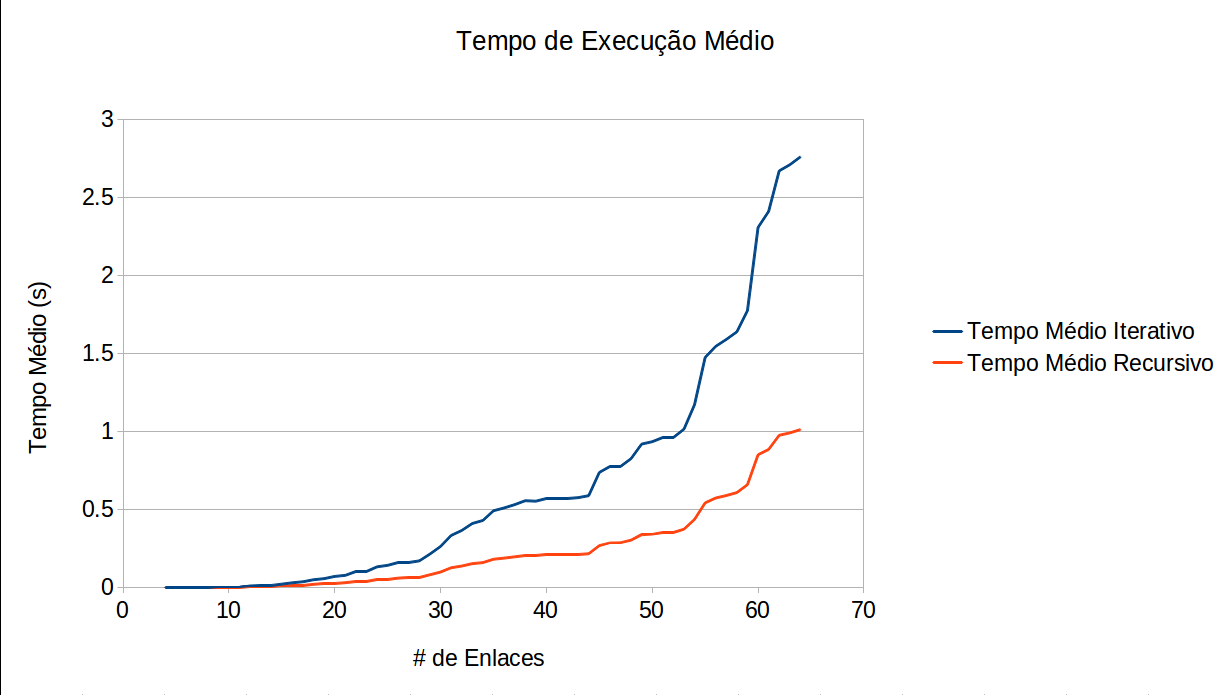
\includegraphics[width=1\linewidth]{figs/tempo64.png} 
    \caption{$n=64$} 
    \vspace{4ex}
  \end{minipage}%% 
  \begin{minipage}[b]{0.5\linewidth}
    \centering
    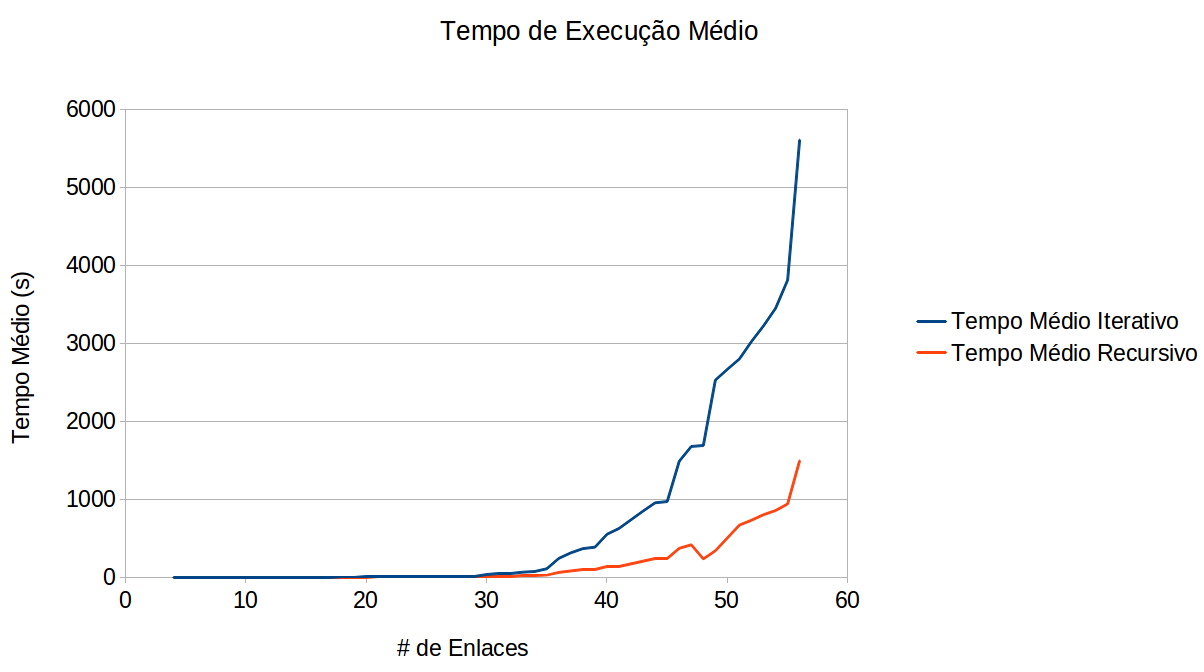
\includegraphics[width=1\linewidth]{figs/tempo128.png} 
    \caption{$n=128$} 
    \vspace{4ex}
  \end{minipage} 
\end{figure}

%A Figura \ref{fig:tempo} mostra um gráfico para cada valor de n. Eles mostram o tempo de execução médio para ambos os algoritmos em função de m.

O primeiro fato a ser notado é que o algoritmo RECURSIVO obteve menores tempos de execução para todos os valores de $n$. Isso reflete a menor complexidade de tempo teórica que o algoritmo RECURSIVO tem em comparção com o algoritmo ITERATIVO, conforme evidenciada na Tabela \ref{table:complexidade}. 

No caso mais complexo, $n=128$ e $m=56$, o tempo para enumerar os conjuntos viáveis no algoritmo ITERATIVO foi de 5612 segundos (aproximadamente, 1 hora e meia), enquanto que para o algoritmo RECURSIVO foi de 1496 segundos (aproximadamente, 25 minutos). Baseando-se em sua aplicação para ajudar a resolver o problema de escalonamento de enlaces mencionado no Capítulo \ref{cap:introducao}, ambos os algoritmos oferecem um tempo de execução aceitável e, portanto, justificam sua implementação.

\section{Conclusão}

Nesse capítulo, a redução da complexidade computacional de $O(m)$ para $O(n)$ em algoritmos que iteram sobre os enlaces de um conjunto foi justificado através de técnicas de otimização. Em seguida, foi descrito um panorama sobre as técnicas de implementação e ambiente utilizados. 

Finalmente, usou-se o resultado das simulações para entender qual o impacto das complexidades computacionais teóricas quando os algoritmos são utilizados na prática. Além disso, também foi possível verificar o tamanho de $|F|$ em função de $m$, que permitiu concluir a superioridade dos algoritmos aqui apresentados em relação aos algoritmos baseados em força bruta pura.
